\documentclass[a4paper,12pt]{article}
%\usepackage{fullpage}
%\usepackage{pdfpages}

\usepackage{geometry}
 \geometry{
 a4paper,
 total={170mm,257mm},
 left=20mm,
 top=20mm,
 }

\usepackage{color}
\usepackage{amsmath,graphicx,makeidx}
\usepackage{lscape}
\usepackage{fancyhdr}
\addtolength{\headheight}{1.5cm} % make more space for the header
\pagestyle{fancyplain} % use fancy for all pages except chapter start
\lhead{
\includegraphics[height=1.7cm]{FOSSEE-logo}} % left logo
\rhead{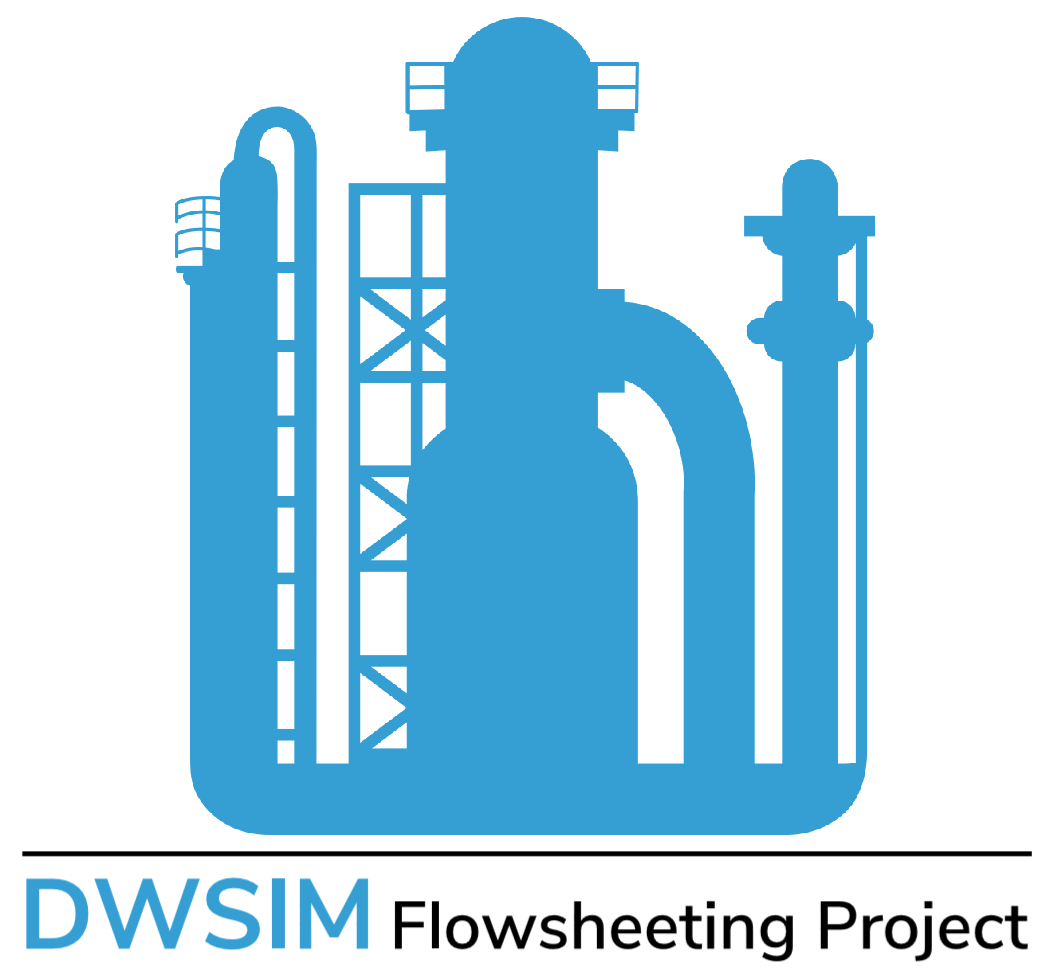
\includegraphics[height=3.5cm]{DWSIM-flowsheeting-project-logo}} % right logo
\renewcommand{\headrulewidth}{0pt} % remove rule below header

\title{Solid Carbon Combustion}
\author{Daniel Wagner \\ DWSIM Developer}
\date{}

\begin{document}

\maketitle

\noindent \textbf{Background \& Description:}
\newline Combustion, or burning, is a high-temperature exothermic redox chemical reaction between a fuel (the reductant) and an oxidant, usually atmospheric oxygen, that produces oxidized, often gaseous products, in a mixture termed as smoke. Combustion in a fire produces a flame, and the heat produced can make combustion self-sustaining. Combustion is often a complicated sequence of elementary radical reactions. Solid fuels, such as wood and coal, first undergo endothermic pyrolysis to produce gaseous fuels whose combustion then supplies the heat required to produce more of them. Combustion is often hot enough that incandescent light in the form of either glowing or a flame is produced.
In this process, solid carbon mixed with air at 298.15 K and 101325 Pa is sent to a conversion reactor. Reaction takes place between carbon and oxygen to form carbon dioxide where 100\% conversion is considered for carbon.

\vspace{25mm}
\centerline{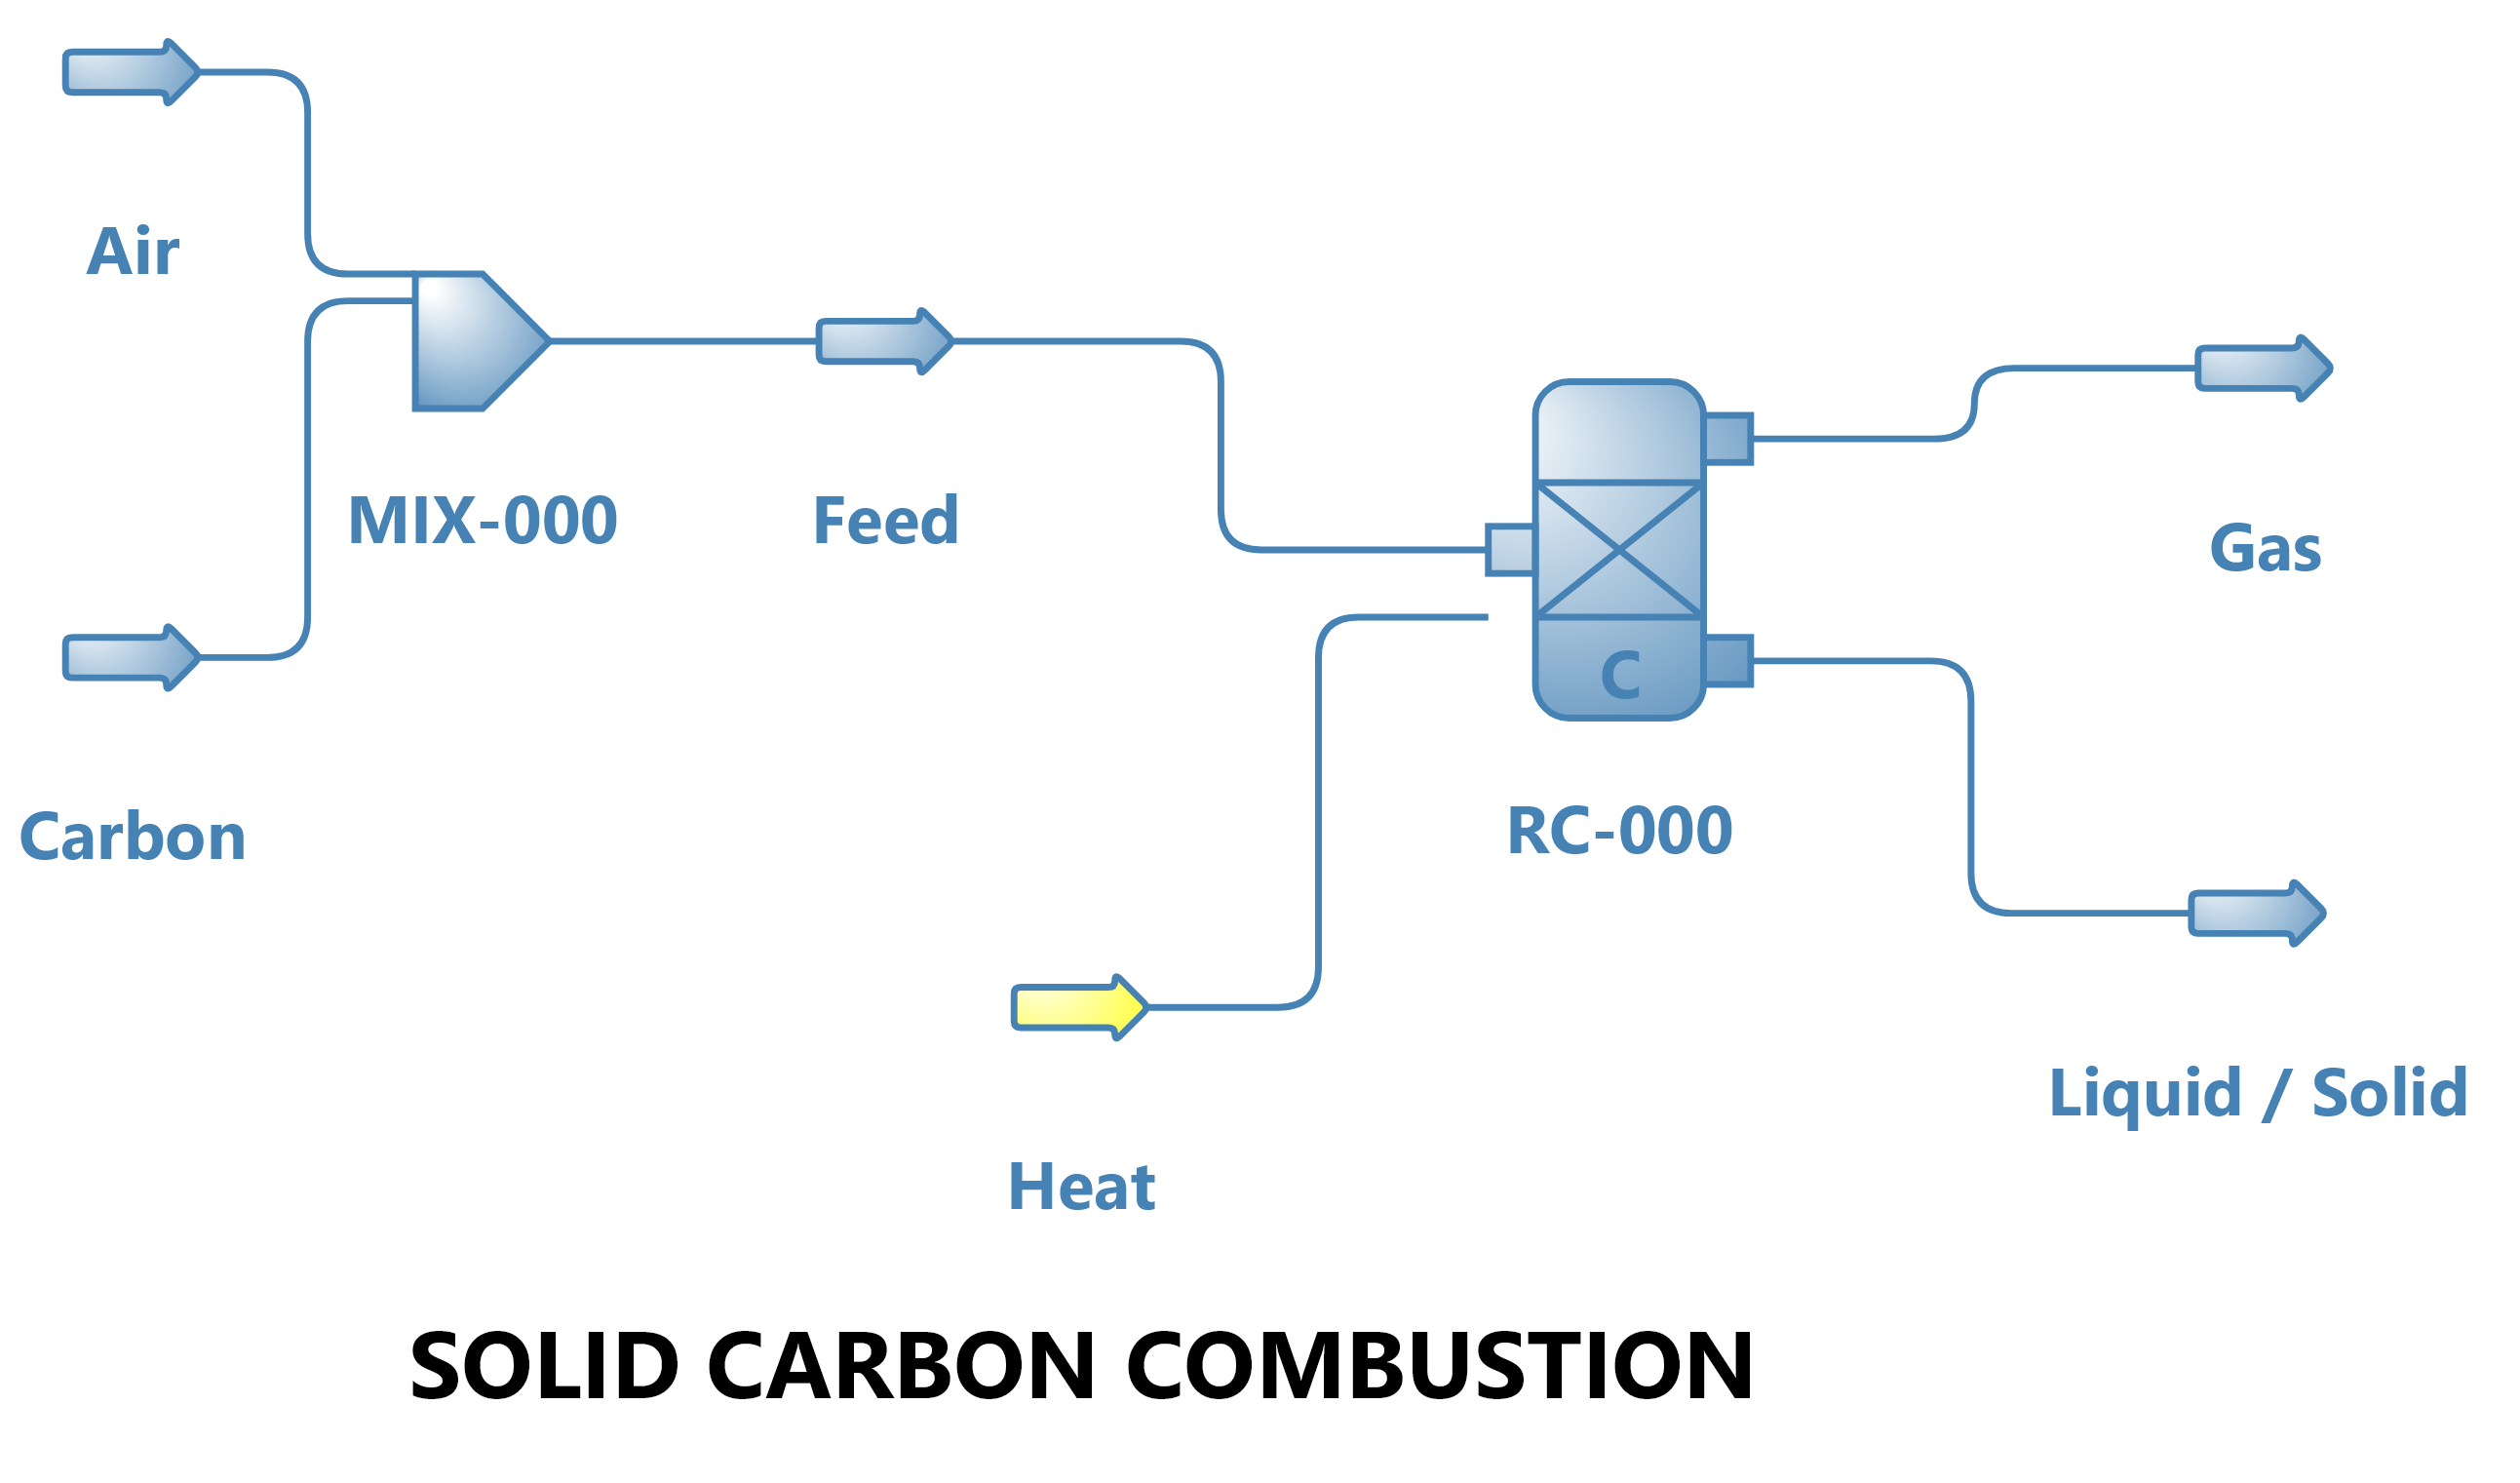
\includegraphics[width=1\linewidth]{Carbon-Combustion.png}}

\newpage
\noindent \textbf{Results:}
\begin{table}[ht]
\centering
\resizebox{\textwidth}{!}{%
\begin{tabular}{|l|l|l|l|l|l|l|}
\hline
Object                                         & Liquid / Solid & Gas       & Feed        & Carbon      & Air       &               \\ \hline
Temperature                                    & 298.15         & 298.15    & 298.15      & 298.15      & 298.15    & K             \\ \hline
Pressure                                       & 101325         & 101325    & 101325      & 101325      & 101325    & Pa            \\ \hline
Mass Flow                                      & 0.005332       & 0.300224  & 0.305556    & 0.027778    & 0.277778  & kg/s          \\ \hline
Molar Flow                                     & 0.399297       & 9.597106  & 11.998313   & 2.312906    & 9.685407  & mol/s         \\ \hline
Mixture Specific Enthalpy                      & -1671324.74    & -0.315341 & -216808.95  & -2384880.36 & -0.239059 & kJ/kg         \\ \hline
Mixture Specific Entropy                       & -4736.77       & 0.132923  & -614.346351 & -6,59.41    & 0.172224  & kJ/{[}kg.K{]} \\ \hline
Molar Fraction (Mixture)  /  Carbon dioxide    & 0.000635       & 0.208565  & 0           & 0           & 0         &               \\ \hline
Mole Fraction (Solid Phase)  /  Carbon dioxide & 0              & 0         & 0           & 0           & 0         &               \\ \hline
Molar Fraction (Mixture)  /  Nitrogen          & 0.000009       & 0.784699  & 0.627661    & 0           & 0.777548  &               \\ \hline
Mole Fraction (Solid Phase)  /  Nitrogen       & 0              & 0         & 0           & 0           & 0         &               \\ \hline
Molar Fraction (Mixture)  /  Oxygen            & 0              & 0         & 0.166847    & 0           & 0.20669   &               \\ \hline
Mole Fraction (Solid Phase)  /  Oxygen         & 0              & 0         & 0           & 0           & 0         &               \\ \hline
Molar Fraction (Mixture)  /  Water             & 0.220416       & 0.006736  & 0.012724    & 0           & 0.015762  &               \\ \hline
Mole Fraction (Solid Phase)  /  Water          & 0              & 0         & 0           & 0           & 0         &               \\ \hline
Molar Fraction (Mixture)  /  Carbon            & 0.77894        & 0         & 0.192769    & 1           & 0         &               \\ \hline
Mole Fraction (Solid Phase)  /  Carbon         & 1              & 1         & 1           & 1           & 0         &               \\ \hline
\end{tabular}%
}
\caption{Streamwise Results for Solid Carbon Combustion}
\end{table}

\end{document}


